\documentclass[answers]{exam}
\renewcommand{\solutiontitle}{\noindent\textbf{}\par\noindent}

\usepackage{fullpage} % Package to use full page
\usepackage{parskip} % Package to tweak paragraph skipping
\usepackage{tikz} % Package for drawing
\usepackage{amsmath}
%\usepackage{hyperref}
\usepackage{graphicx}
\usepackage{enumerate}
\usepackage{caption}
\usepackage{subcaption}
\usepackage{multicol}
\usepackage{mathptmx}
\usepackage{amsmath}
\usepackage{amssymb}
\usepackage{nameref}
\newcommand{\mypoints}[1]{\textcolor{red}{(#1 points)}}
\newcommand{\myinput}[1]{\textcolor{blue}{#1}}

\title{\normalfont \normalsize 
\textsc{{Department of Computer Science, UCLA \\
CS 188-2: Introduction to Computer Vision}}
\date{\vspace{-12ex}}
}
\begin{document}
\maketitle
\rule{\linewidth}{0.8pt} \\[6pt] 
\noindent
\large\textbf{\textsc{Instructor:}} Prof. Fabien Scalzo \hfill \large\textbf{\textsc{Name:}} \myinput{Insert Your Name}\\
\large\textbf{\textsc{TA:}} Albert Zhao\hfill 
\large\textbf{\textsc{UID:}} \myinput{ Insert Your UID}
\rule{\linewidth}{0.8pt} \\[6pt] 

\begin{center}
{\normalsize \textsc{Homework 2: Synthetic Aperture Imaging} } \\
{\normalsize Deadline: Friday, November 15, 11:59 pm} 
\end{center}
\vspace{2cm}

\begin{table}[h]
\centering
\resizebox{1.0\textwidth}{!}{%
\begin{tabular}{clccc}
\hline
\multicolumn{1}{c}{\textsc{Problem}} & \multicolumn{1}{c}{\textsc{Topic}} & \multicolumn{1}{c}{\textsc{Max. Points}} & \multicolumn{1}{c}{\textsc{Graded Points}} & \multicolumn{1}{c}{\textsc{Remarks}} \\  \hline \\ 
 \ref{sssec:staticscene} & Set up a Static Scene &  0.5 &  &  \\ [2mm]
 \ref{sssec:4dlf} & Capture a 4D Light Field  & 0.5 &  &  \\ [2mm]
 \ref{sssec:dataproc} & Acquiring the Data & 0.5 &  &  \\ [2mm]
 \ref{sssec:tempwindow} & Template and Window & 0.5 &  &  \\ [2mm]
 \ref{sssec:normcorr} & Normalized Cross Correlation &  0.5 &  &  \\ [2mm]
 \ref{sssec:pixshift} &  Retrieving the Pixel Shifts &  0.5 &  &  \\ [2mm]
 \ref{sssec:synthesis} & Synthesizing an Image with Synthetic Aperture & 1.0 &  &  \\ [2mm]
 \ref{sssec:resynthesis} & Repeating the Experiment for Different Templates & 1.0 &  &  \\ [2mm]
 \ref{sssec:derivation} & Deriving the Blur Kernel Width  & 3.0 &  &  \\ [2mm]
 \ref{sssec:kernelshape} &  Blur Kernel Shape & 1.0 &  &  \\ [2mm]
\ref{sssec:scenedepth} & Blur and Scene Depth & 0.5 &  & \\ [2mm]
 \ref{sssec:focallength} & Blur and Focal Length & 0.5 &  & \\ [2mm] \hline \\ 
    & \textbf{Total} & 10 & & \\ [2mm]\hline
\end{tabular}
}
\caption*{}
\label{}
\end{table}

\newpage

\section{Motivation}
 \emph{At the top-level, this problem set enables you to turn your cell phone into a 4D light field camera}. 
 
Shallow depth of field, i.e. having only a small area in focus, is a desirable aesthetic quality in a photograph. Unfortunately, this effect requires a large aperture, i.e., the lens is going to be big and bulky! But what if it was possible to turn your cell phone into a camera with a large aperture? What if we could selectively focus on objects in post-processing?

The goal of this homework is to synthesize images with smaller depths of field thus making it appear to have been taken from an expensive camera with a larger
aperture\cite{Lumsdaine09thefocused} \cite{Levoy}. Figure \ref{pset_motivation}a and b show a scene image with the corresponding synthetic aperture image with lower depth of field. 

\begin{figure*}[h]
\begin{multicols}{2}

	\captionsetup{justification=centering}
    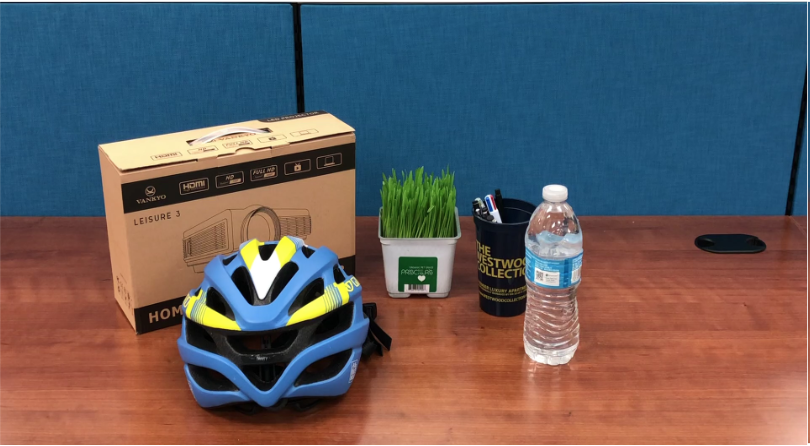
\includegraphics[width=0.5\textwidth]{pset_scene.png} \caption*{(a) All-in focus image.}\par 
    \captionsetup{justification=centering}
    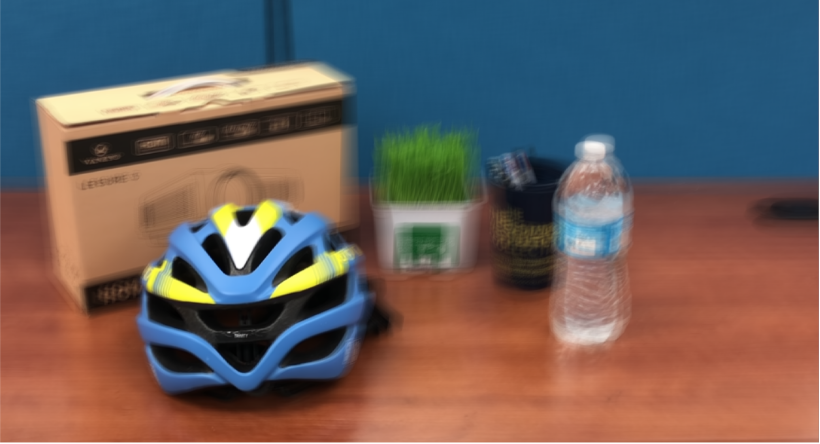
\includegraphics[width=0.5\textwidth]{pset_output_2.png} \caption*{(b) Post-processed to blur the background}\par 
    \end{multicols}
    \caption{\textbf{Turning a cell phone into a light field camera.} (a) An all-in focus image taken with a cell phone camera. (b) A light field stack is post-processed to blur out the background. Notice how the helmet stands out from the background.}
    \label{pset_motivation}
\end{figure*}

\section{Experimental Component}

We will capture a video by moving the camera in a zig-zag path as shown in Figure \ref{camera_motion} in front of the static scene. Please use Python for all codes. Fill in each box below for credit.\\


\begin{figure*}[h]
\centering

    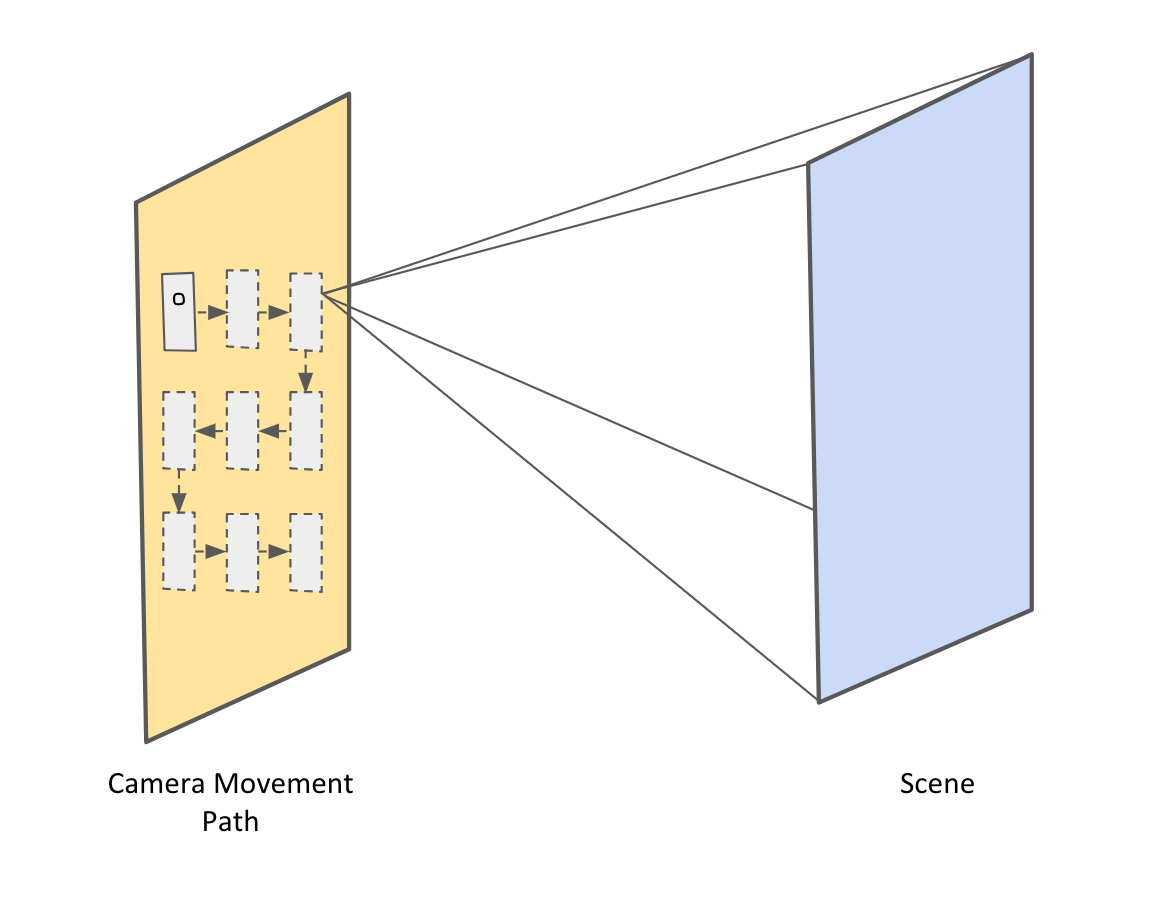
\includegraphics[width=0.75\textwidth]{pset_camera_motion.png}
    \captionsetup{justification=centering}
    \caption{A zig-zag planar motion of the camera in front of the static scene to capture a video.}
    \label{camera_motion}
\end{figure*}

Please note:
\begin{enumerate}
\item The algorithm being implemented does not take camera tilt into account. Avoid tilting and rotating the camera as much as possible. 
\item The instruction set use a planar zig-zag path for camera motion as in \ref{camera_motion}. However, you are allowed to try different paths like circular or polyline.
\item The number of frames in the video captured will determine the time required to compute the output. Make sure the video is not too long.
\end{enumerate}


\subsection{Set up a Static Scene \mypoints{0.5} } \label{sssec:staticscene}
Set up a static scene similar to the one shown in Figure \ref{pset_motivation}a. Try to have objects at different depths. For credit, place your image in the box below (replace our helmet scene with your own scene).  

\begin{solution}
\centering 
  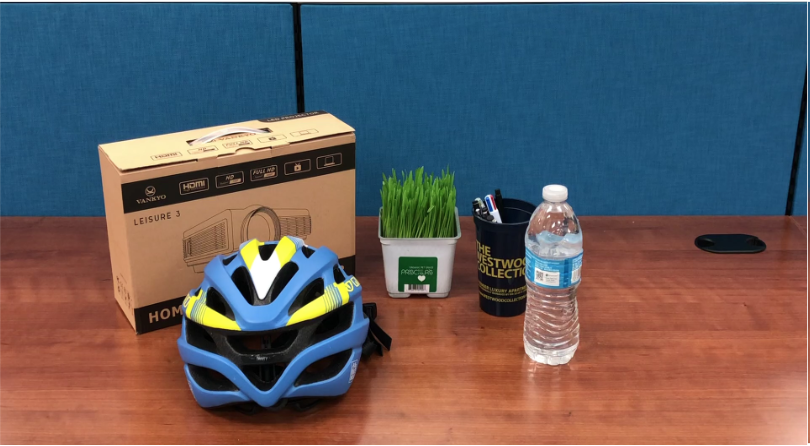
\includegraphics[width=0.5\textwidth]{pset_scene.png}
  \captionof{figure}{\myinput{Insert an ordinary photograph of the scene (replace our example).}}
\end{solution}

\subsection{Capture a 4D Light Field \mypoints{0.5}}\label{sssec:4dlf}
Take a video by waving your camera in front of the scene by following a specific planar motion. The more you cover the plane, the better will be your results.
Ensure that all objects are in focus in your video. For credit, place three frames of the video in the box below (replace our example). These frames differ in their \emph{parallax}, i.e., an effect where object positions change in response to view.
\begin{solution}
\centering 
  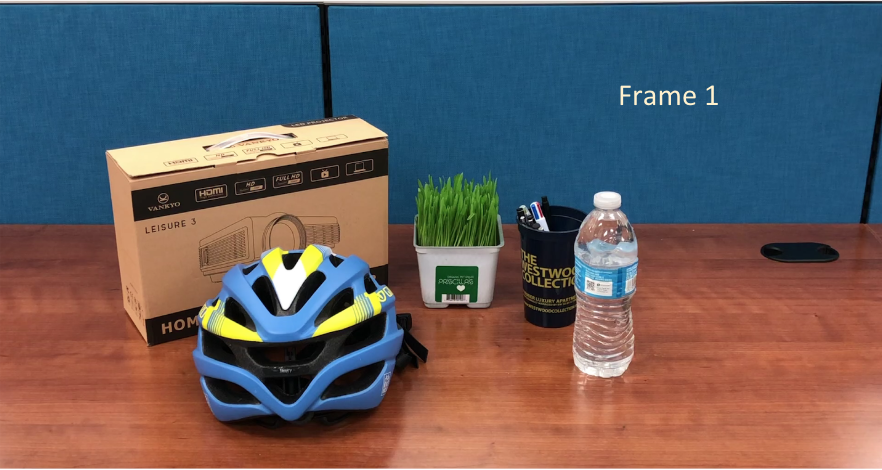
\includegraphics[width=0.5\textwidth]{pset_frame1.png}
  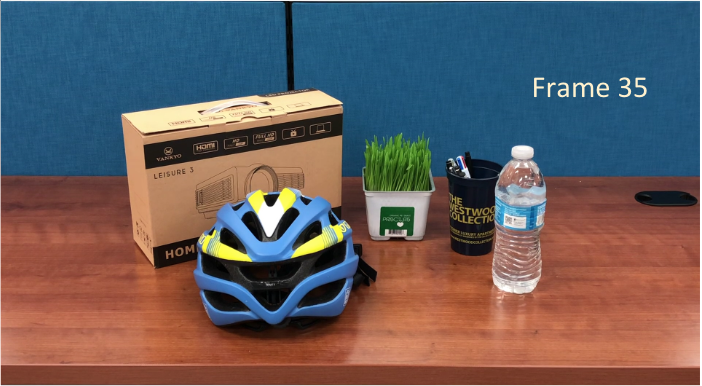
\includegraphics[width=0.5\textwidth]{pset_frame35.png}
  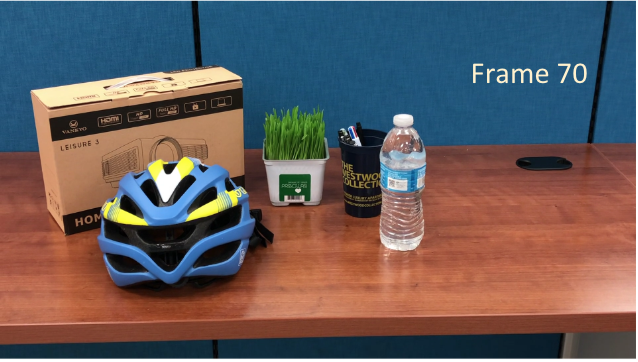
\includegraphics[width=0.5\textwidth]{pset_frame70.png}
  \captionof{figure}{\myinput{Insert any three frames of your video here (replace our example). Make sure there is sufficient parallax in the images.}}
\end{solution}
\newpage
\subsection{Acquiring the Data \mypoints{0.5} }\label{sssec:dataproc}
Write a function to read your video file and convert the video into a sequence of frames. Since this was captured from a cell phone, each frame image is in RGB color. Write a script to convert each frame to gray-scale. For credit, place the gray scale image of the first frame of your video in the box below (replace our example). 
\begin{solution}
\centering 
  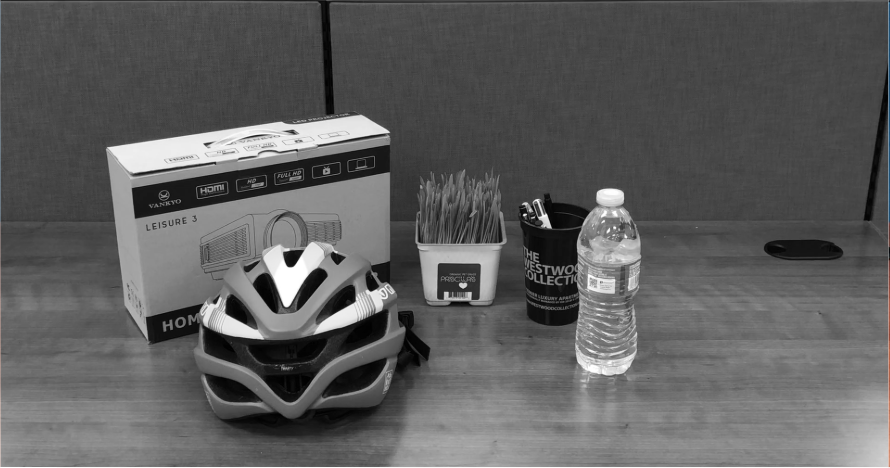
\includegraphics[width=0.5\textwidth]{pset_frame1_grayscale.png}
  \captionof{figure}{\myinput{Insert the gray-scale image of the first frame (replace our example).} }
\end{solution}

\subsection{Registering the Frames \mypoints{1.5} } \label{sssec:regframes}


\subsubsection{Template and Window \mypoints{0.5} } \label{sssec:tempwindow}


From the first frame of your video, select an object as a template. We will be registering all other frames of the video with respect to this template. Once a template has been selected in the first frame, we search for it in the subsequent frames. The location of the template in a target frame image will give us the shift(in pixels) of the camera. Since we don't have to search for the template in the entire target frame image, we select a window to perform this operation. Note, however, that selecting a window is optional. This is done just to reduce the computation time. For credit, place the image of the first frame of your video in the box below with the template and the window markings (replace our example). 
\begin{solution}
\centering 
  
  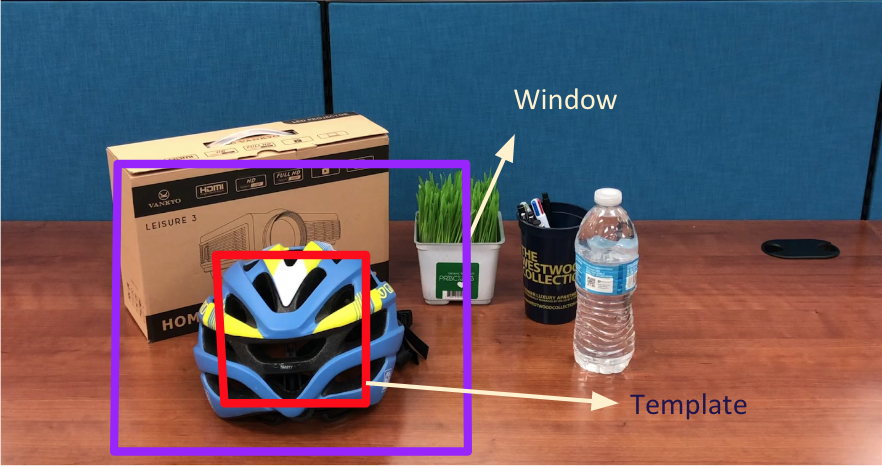
\includegraphics[width=0.5\textwidth]{pset_window_2.png}
  \captionof{figure}{\myinput{Insert your image with template object and search window marked (replace our example). }}
\end{solution}



\subsubsection{Normalized Cross Correlation \mypoints{0.5} }\label{sssec:normcorr}



Perform a normalized cross correlation of the template with the extracted search window.


Let $A[i,j]$ be the normalized cross-correlation coefficient. If $t[n,m]$ is our template image and $w[n,m]$ is our window, then from \cite{Lewis95fastnormalized} we have:

\begin{equation}
A[i,j] = \frac{\sum_{n,m=1}^T [w(n,m) - \overline{w}_{i,j}] [t(n-i, m-j) - \overline{t } ]}{ \{\sum_{n,m=1}^T [w(n,m) - \overline{w}_{i,j}]^2 \sum_{n,m=1}^T [t(n-i, m-j) - \overline{t } ]^2 \}^{0.5}},
\end{equation}

where $\overline{t}$ is the mean of the template and $\overline{w}_{i,j}$ is the mean of the window $w[n,m]$ in the region under the template. Plot the cross correlation coefficient matrix $A[i,j]$ for one of the frames. For credit, place the plot in the box below (replace our example).


\begin{solution}
\centering 
  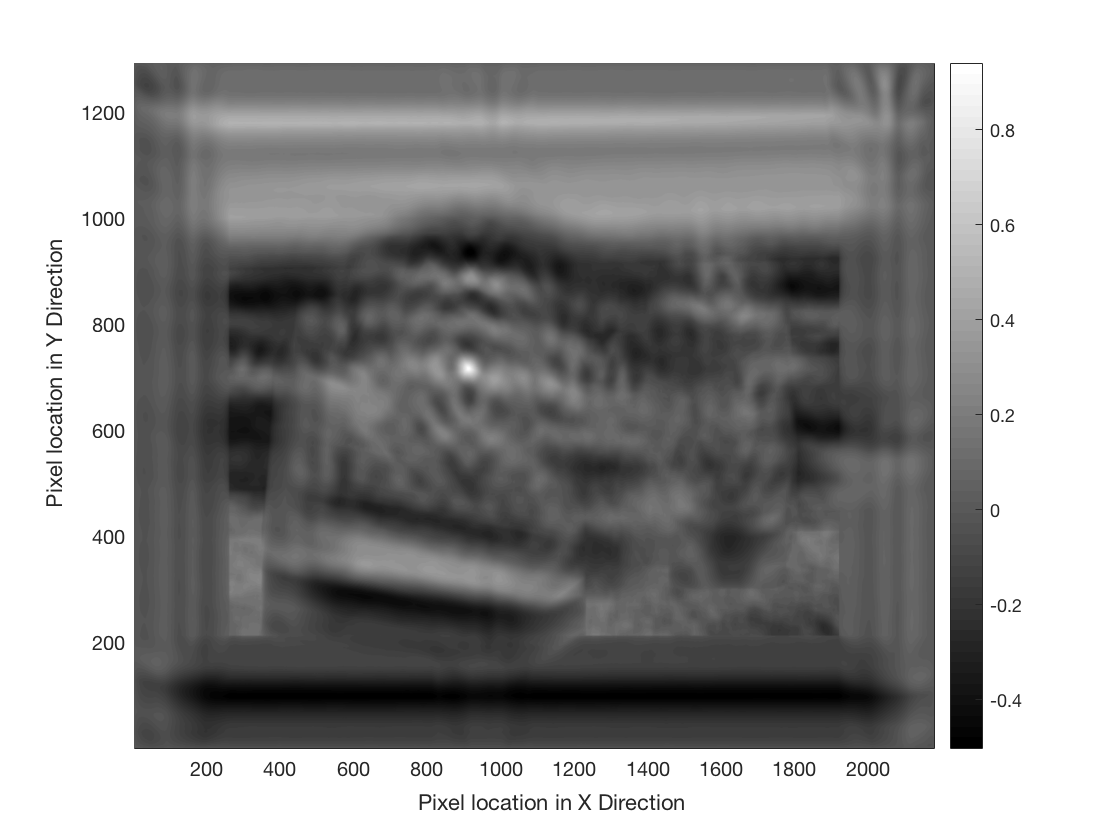
\includegraphics[width=0.5\textwidth]{pset_normcorr.png}
  \captionof{figure}{\myinput{Insert the plot of the correlation coefficient Matrix (replace our example).}}
\end{solution}


[Hint: Use the Scikit-image function match\_template with pad\_input=True to perform the 2D cross correlation. Scikit-image, an image processing library, can be installed via pip.]

\subsubsection{Retrieving the Pixel Shifts \mypoints{0.5} }\label{sssec:pixshift}


The location that yields the maximum value of the
coefficient $A[i,j]$ is used to compute the shift \cite{Georgeiv_lightfield}. The shift in pixels for each frame can be found by: 

\begin{equation}
[s_x, s_y] = max_{i,j} \{A[i,j]\}.
\end{equation}
For credit, please place the plot of $s_x$ v/s $s_y$ in the box below (replace our example).
\begin{solution}
\centering 
  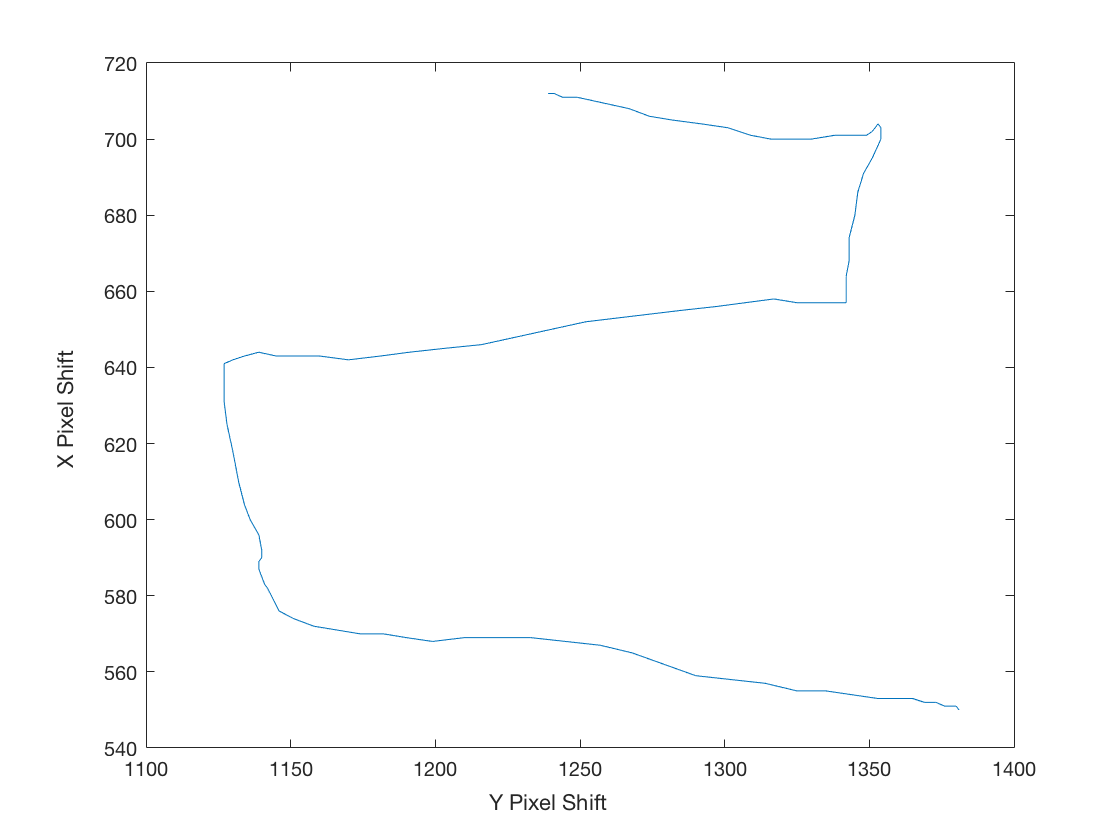
\includegraphics[width=0.5\textwidth]{pset_path.png}
  \captionof{figure}{\myinput{Insert the plot of X pixel shift v/s Y pixel shift (replace our example).}}
\end{solution}

\subsection{Synthesizing an Image with Synthetic Aperture \mypoints{1.0} }
\label{sssec:synthesis}
Once you have the pixel shifts for each frame, you can synthesize refocused image by shifting each frame in the opposite direction and then summing up all the frames. (Note: in Section~\ref{assessment}, you will need to explain why this operation works. Start thinking about this now!) 

Suppose the pixel shift vector for Frame Image $I_i[n,m]$ is $[s_{x_i}, s_{y_i}]$. Then, the image output, $P[n,m] $ with synthetic aperture is obtained as:

\begin{equation}
P[n,m] = \sum_i I_i[n-s_{x_i}, m-s_{y_i}].
\end{equation}

For credit, place your synthetically "defocused" image in the box below (replace our example). 

\begin{solution}
\centering 
  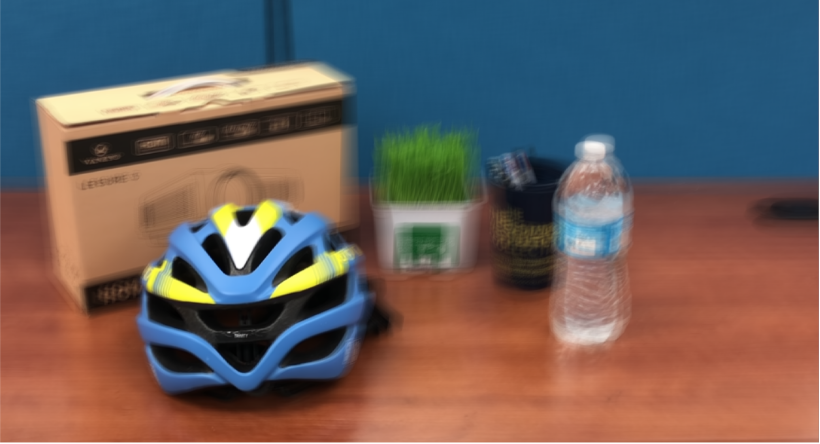
\includegraphics[width=0.5\textwidth]{pset_output_2.png}
  \captionof{figure}{\myinput{Insert an image with an object in synthetic focus (replace our example).}}
\end{solution}
[Hint: Use the OpenCV function warpAffine with a transformation matrix corresponding to a translation to perform the shifting operation.]

\subsection{Repeating the Experiment for Different Templates \mypoints{1.0} } \label{sssec:resynthesis}

Now, we will exploit the fact that we can synthetically focus on different depths. To do this, select a new object as your template and repeat all the steps to generate an image that is focused on this new object. Here, we have selected the cup as our new object. For credit, place a de-focused image with a different template object in focus in the box below (replace our example). 

\begin{solution}
\centering 
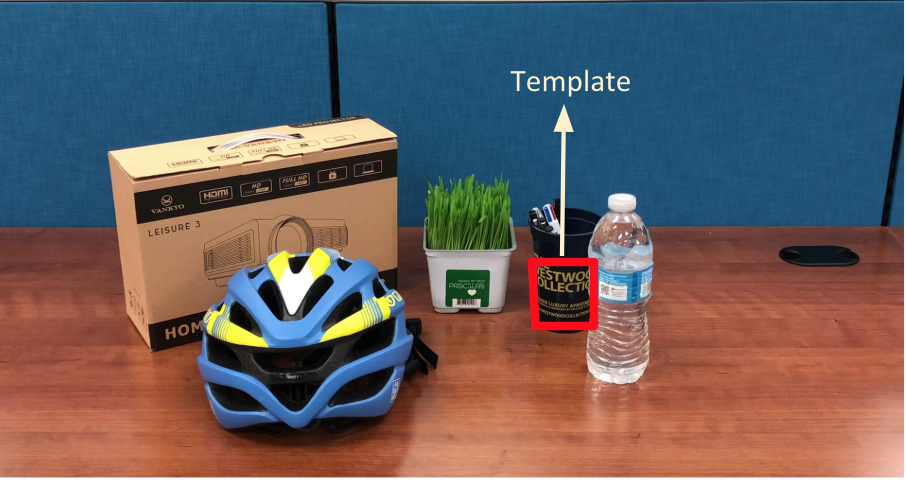
\includegraphics[width=0.5\textwidth]{pset_template.png}
  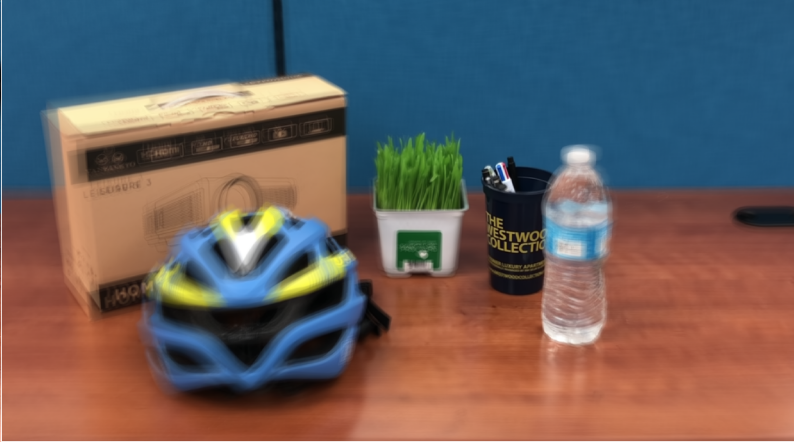
\includegraphics[width=0.5\textwidth]{pset_output.png}
  \captionof{figure}{\myinput{Insert an image with an object in synthetic focus. This object should be different from the previous box (replace our example).}}
\end{solution}


\newpage
\section{Assessment}
\label{assessment}

\subsection{Deriving the Blur Kernel Width \mypoints{3.0}}\label{sssec:derivation}

The goal is to understand how much blur is synthetically added by using a model of pinhole cameras. Consider the coordinate diagram shown in Figure \ref{assesment}. Here, [$X_1$,$Z_1$] is a scene point of an object in the template, [$X_2$,$Z_2$] is a scene point of an object in the background and $C^{(i)}$ for $i=1,\ldots,k$ are positions of the apertures of cameras at which the scene is captured. The maximum camera translation is $\Delta$ and $f$ is the focal length of the cameras (all are assumed to be the same).

\begin{figure*}[h]
\centering

    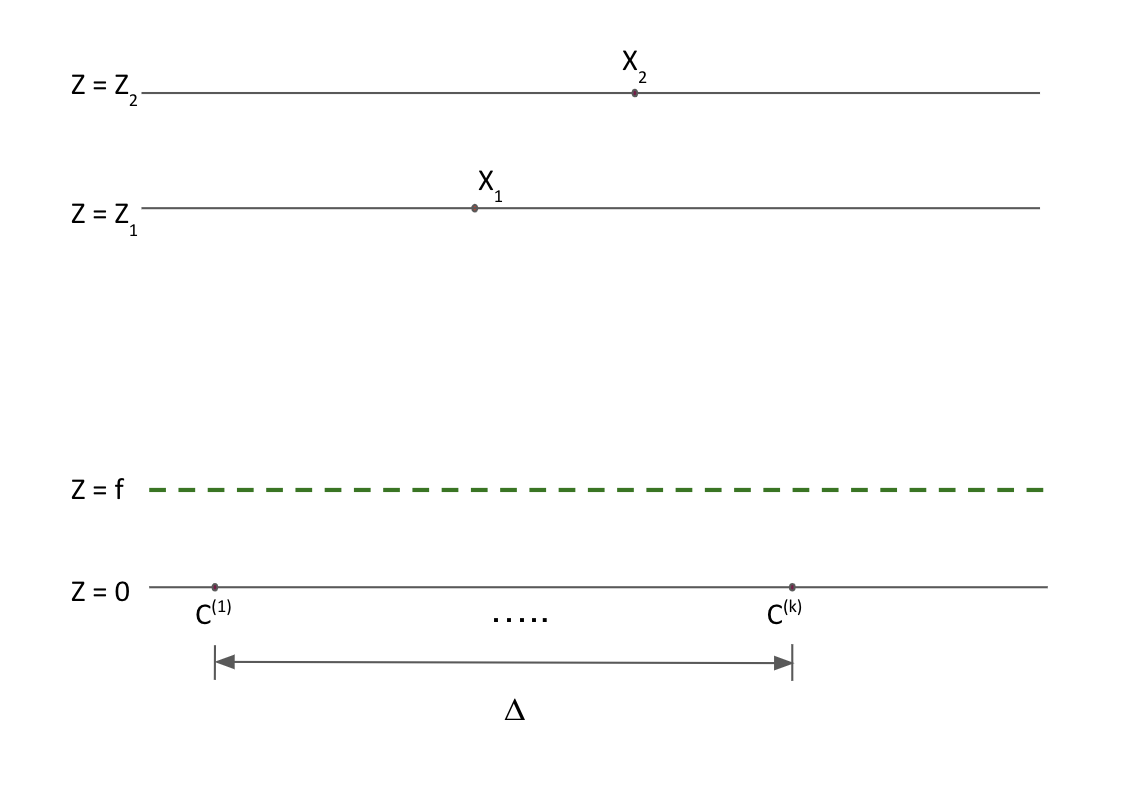
\includegraphics[width=0.9\textwidth]{pset_assesment.png}
    \caption{Example coordinate system and notation. In this figure, the dashed plane is the virtual film plane, placed one focal length \emph{above} the apertures located at $C^{(1)},\ldots,C^{(k)}$. This is a common shorthand convention so we do not have to flip the camera images. In reality, the actual film plane would be one focal length below the aperture location. This coordinate system is used as a guide - you are welcome to modify as needed.} 
    \label{assesment}
\end{figure*}


We will use the shift-and-add method for light field imaging such that $X_1$ is the point in focus (i.e. as the "template" that we "shift and add"). Derive a mathematical expression for the full-width half maximum (FWHM) of the blur kernel ($W$) applied to $X_2$. Credit will be assessed both for technical correctness and the presentation of the derivation. You should not need figures, but are welcome to include them. Insert your derivation in the box below. 

[Hint: Our solution to derive $W$ was about a half page.]

[Hint: To check your solution, if $Z_1 = Z_2$ the width of the blur kernel should be zero.]



    \begin{solution}
    \vspace{20cm} %remove this
    \end{solution}

\subsection{Blur Kernel Shape \mypoints{1.0}} \label{sssec:kernelshape}

Now that you have derived the FWHM of the blur kernel, please write the functional expression for the blur kernel. For example, is it a Gaussian blur?
    \begin{solution}
    \vspace{3cm} %remove this
   \myinput{} 
    \end{solution}
    
\subsection{Blur and Scene Depth \mypoints{0.5}} \label{sssec:scenedepth}

Plot the width of the blur kernel, $W$, as a function of the difference in depth planes, $\lvert Z_2 - Z_1 \rvert$. Insert your plot in the box below. Comment on the relationship between these variables. 
    \begin{solution}
    \vspace{3cm} %remove this
   \myinput{} 
    \end{solution}


\subsection{Blur and Focal Length \mypoints{0.5}} \label{sssec:focallength}

Plot the width of the blur kernel, $W$, as a function of the focal length of the camera, $f$. Insert your plot in the box below. Comment on the relationship between these variables.

    \begin{solution}
    \vspace{3cm} %remove this
   \myinput{} 
    \end{solution}

\newpage

\section{Submission}

Your submission will consist of a single tarball, "UID.tar.gz", where UID is the university ID of the submitter. It will be submitted on CCLE. Your tarball will consist of several files, listed below. Please respect the filenames and formatting \textbf{exactly}. You tarball should include:
\begin{itemize}
    \item README: a .txt file
        \begin{itemize}
            \item Line 1: Full name, UID, email address of first group member (comma separated)
            \item Line 2: Full name, UID, email address of second group member (comma separated) if any, empty otherwise
            \item Use the rest of the file to list the sources you used to complete this project
        \end{itemize}
    \item code/: a directory containing all the .py files that you used for your project. There are no requirements as to how the code files are formatted.
    \item HW2: a PDF file with the answers to the questions in the homework.
\end{itemize}

\textbf{Note:} Your tarball should not contain the video used for the experimental component.


\bibliographystyle{plain}
\bibliography{bibliography.bib}


\end{document}